
\chapter{\rnn{} Performance}%
\label{sec:off_ana}

This section is dedicated to a more detailed assessments of the \rnn{} behavior 
in the period 2017-2018 with respect to the previous electron trigger cut-based strategy.
Using \Zee{} \tnp{} selection, the agreement between the two triggers and
possible biases, caused by the introduction of the \rnn{} using the variables
employed by the likelihood algorithm, were investigated
Since offline and final HLT electron
selections are based on such variables, limiting the evaluation to them suffice
to understand any possible impact of the \rnn{} algorithm in most analyses.
Additionally, these variables are interesting since they compact the input space
in a set of few variables with low correlation and high interpretability power. 
%One should keep in mind that the \rnn{} algorithm had access only to the ring description during Run~2 operation.

As indicated in Table~\ref{tab:quadrant_vs_agreement}, two analyses were performed to assess the
trigger performance with and without \rnn{}, when applied to the tag (Agreement Analysis) and
to the probe (Quadrant Analysis). The Tag \& Probe events have one probe electron that was not 
used to decide the selection of that event at the trigger level.


\begin{table}[ht!]\footnotesize
\centering
\caption{Customized \Zee{} \tap{} selection criteria employed in the
agreement and quadrant analyses in the Run 2 (2017-2018 period)}.%
\label{tab:quadrant_vs_agreement}
\resizebox{\textwidth}{!}{%
  \begin{tabular}{p{2cm}p{4.5cm}p{5.5cm}}
\hline
\hline
\hline
& Agreement Analysis (Section~\ref{ssec:agreement}) & Quadrant Analysis
(Section~\ref{ssec:quadrant}) \\
\hline
\hline
tag (and event) & trigger selection comparison & primary lowest unprescaled electron triggers \\
\hline
probe & \vloose & trigger selection comparison with offline selection fixed to
the same trigger requirement \\
\hline
\hline
\hline
\end{tabular}
}
\end{table}

The Quadrant Analysis allows to directly assess possible bias caused by the
introduction of the \rnn{} by comparing the profiles for all possible disjoint
decisions from the two trigger classifiers. Hence, it is possible for the classifiers
to agree by both accepting or rejecting the event. Likewise, they are able to
disagree in two possible cases where either one decides to accept the event
while the other rejects it.

Although it is reasonable to expect that the shower development of the tag and
the probe are independent from each other, and that the \rnn{} when applied to
the tag selection cannot, in principle, alter the profile of the probes besides
changing the number of \tnp{} pairs. Such evaluation of any possible systematic effect caused by the introduction of the \rnn{} in the extraction of the likelihood PDFs, employed for offline and final HLT selection, is performed by the Agreement Analysis.

\FloatBarrier
\section{Impact on CPU Demands} %\label{ssec:cpu_reduction}

As observed in the efficiency measurements during Run~2 data taking, the \rnn{} allowed more effective \fastcalo{} operation in triggers with electrons above \SI{15}{\GeV}  with respect to the previous cut-based approach. 


%In this section, it was evaluated how the most efficient trigger configuration 
%improved the online system in terms of resource requirements. First, the CPU 
%requirements at the \fastcalo{} level is discussed in~\ref{top:fastcalo_cpu}). Finally, 
%the full impact of CPU requirements of the \rnn{} in a primary electron trigger is evaluated in~\ref{top:cpu_e26}).


%\subsection{Estimated CPU Impact}\label{top:fastcalo_cpu}


The overhead required to computed the NN decision by running a single electron trigger with and without the \rnn algorithm, in two individual non-concurrent executions using the same dedicated node\footnote{It was used a techlab node Xeon Phi 7120 (1.7 GHz, 32 threads) with 256 Gb@1333 of memory and a SL6 OS.}, was evaluated
It should be mentioned that, in order to reduce implementation efforts, electron triggers executing the \rnn{} information compute their information after the cut-based reconstruction, whose decision is not computed. As a result of this, the \rnn{} electron 
triggers always demand additional \fastcalo processing time.

Figures~\ref{fig:fastcalo_fex_time} and~\ref{fig:fastcalo_hypo_time} show the comparison of the total CPU time per event for the feature extraction and hypothesis algorithms in the \fastcalo respectively.
The CPU time does not include the online data preparation time and measurements were evaluated from a very loose selection electron trigger with individual executions in the same dedicated computer node.


The measurement employed events from the enhanced bias (EB)
stream~\cite{eb_description} typically extracted from one hour acquisition with
a specific trigger menu based only on first level selection and aiming at
collecting about one million background events more likely to be accepted by the
\hlt{}. This behavior is obtained by applying an increased weighting in high-\pt{} region,
and at a output trigger rate of \SI{300}{\hertz}~\cite{eb_specifications} for one hour. Hence, the
measurements are performed under pile-up conditions with the execution of the
reconstructed observable algorithm for multiple RoIs in the same bunch-crossing event.


\begin{figure}[h!tb]
	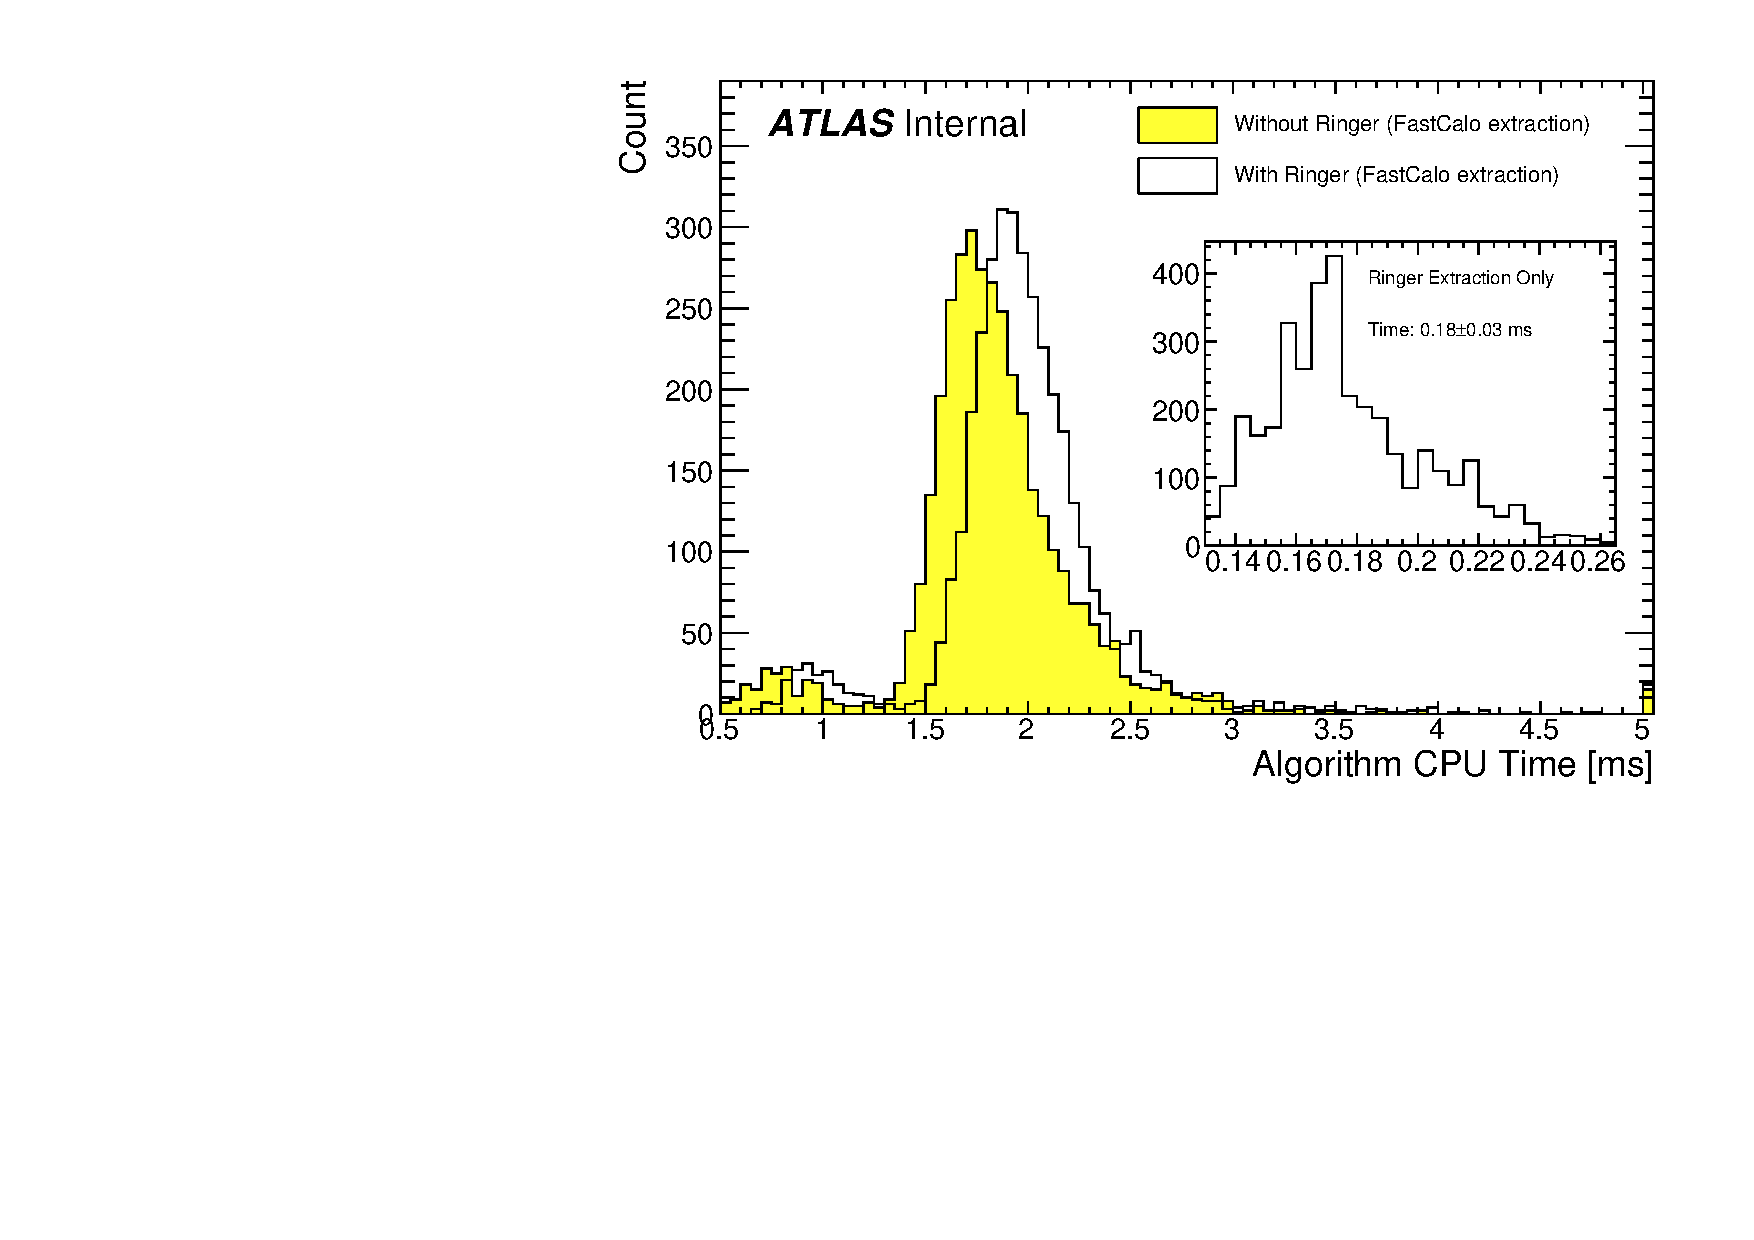
\includegraphics[width=.7\textwidth]{sections/05_analysis/figures/EgammaFex_TotalTime}
	\centering
	\caption{\label{fig:fastcalo_fex_time}
		Total CPU time per event for the feature extraction algorithms in the \fastcalo step of electron rerunning triggers with (white) and without (yellow) \rnn{} using EB events ($\avgmu=45$ peak). Detail on the right shows the CPU time of the ring variable extraction.  
	}
\end{figure}

\begin{figure}[h!tb]
	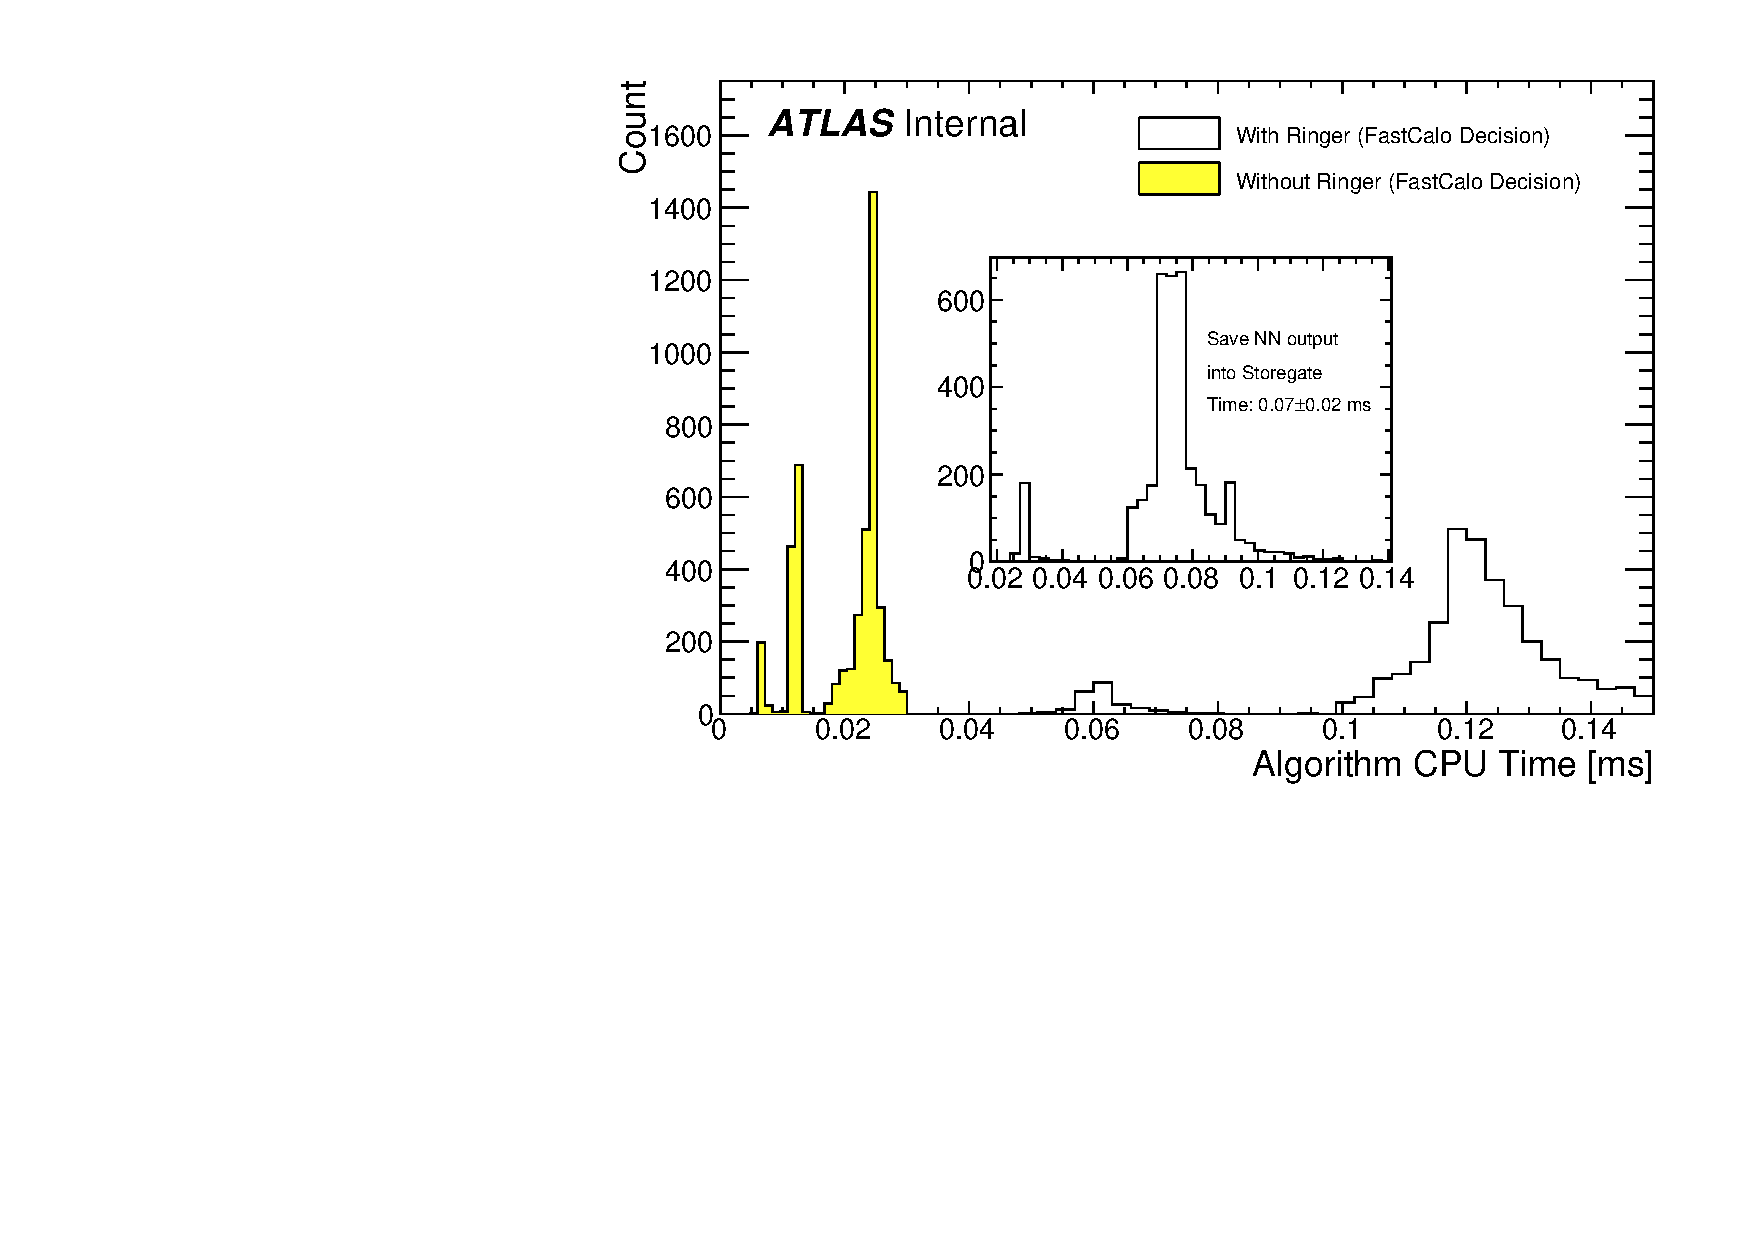
\includegraphics[width=.7\textwidth]{sections/05_analysis/figures/EgammaHypo_TotalTime.pdf}
	\centering
	\caption{\label{fig:fastcalo_hypo_time}
		Total CPU time per event for the hypothesis testing algorithms
		in the \fastcalo step of electron rerunning triggers with (white) and without (yellow) \rnn{} using EB events ($\langle \mu \rangle = 45$ peak). The center histogram represents the CPU time to store the \rnn{} output in persistent file format.}
\end{figure}

A multi-modal structure can be observed in the feature extraction distributions
of both trigger configurations, which is associated to the algorithm
for retrieving the EM2 cells and building related shower shape
variables\footnote{The three peak structure comes from the raw data conversion.
	Particularly, these are amongst the most-demanding contributions to
	the \fastcalo total CPU time.}. The computation of the ring variables, the only difference between the
triggers in the \fastcalo feature extraction, requires an additional average CPU time per
event of \SI{0.18 \pm 0.03}{\ms/\text{event}}. 
A less relevant contribution
comes from hypothesis testing, in which the ring variables are normalized, the
discriminating is computed, compared to the selection requirement and stored into the persistent file format\footnote{For Run-3 this step has been removed as a way to reduce the CPU time at \fastcalo step.}. 
Specifically, \rnn{} hypothesis testing is considerably more demanding
, up to \SI{0.14}{\ms/\text{event}}, mostly due to the time 
to store the neural network output \SI{0.07 \pm 0.02}{\ms/\text{event}}, 
than the cut-based selection
(\SI{0.02}{\ms/\text{event}}), however small with respect to the feature
extraction values. 


Taking into account the referred values, the \rnn{} can require a
relative increase of up to \SI{50}{\%} in the \fastcalo{} CPU time per event
with respect to the trigger without \rnn{}\footnote{It is expected that the result be
	dependent on the trigger configuration due to presence of pile-up. Reported
	results are for e17\_lhvloose\_nod0.}. Nonetheless, the \rnn{} contributes to
a more discriminating selection, allowing to reduce CPU demanding triggers
by reducing the processing of fake electron in subsequent steps that are more computationally demanding.


The potential of saving CPU usage by
avoiding the computation of fake candidates with the \rnn algorithms was demonstrated using algorithms with the lowest-transverse-energy-threshold unprescaled single electron tight trigger. This trigger algorithm was executed with
and without the \rnn{} algorithm using a dedicated node for processing.
In this measurement, where about 3,400 events from the EB stream were considered, the \rnn{} algorithm provided an overall
\SI{60}{\%} reduction (\SI{30.72}{\milli\second} to \SI{10.36}{\milli\second})
in the CPU demands.


\section{Quadrant Analysis}\label{ssec:quadrant}

The Quadrant Analysis was developed to compare the decision of two classifiers. Given signal candidates and two classifiers, these are the possibilities: either both accept or reject the candidates or only one accepts the candidates. The four possible decision quadrants are evaluated from shower shape distributions. Furthermore, in this analysis, it's also possible to compare the disagreement between two classifiers. The disagreement between two classifiers $\textbf{A}$ and $\textbf{B}$ can be defined as:

\begin{equation}
    \text{disagreement} = \frac{N_{\textbf{A}}+N_{\textbf{B}}}{N_{\textbf{A}}+N_{\textbf{B}}+N_{\textbf{AB}}+N_{!\textbf{AB}}}
    \label{eq:disagreement}
\end{equation}
where $N_{\textbf{A}}$ ($N_{\textbf{B}}$) is the total of candidates accepted by classifier $\textbf{A}$ ($\textbf{B}$) and $N_{\textbf{AB}}$ ($N_{\textbf{!AB}}$) is the total of candidates accepted (rejected) by both classifiers.

In this approach, only data collected by the primary triggers whose selection is from its offline equivalent are considered\footnote{I.e., if a \tight{} trigger leg is being evaluated, it also applied the \tight{} offline selection to the candidate.}.
Results in Section~\ref{top:quadrant_results} show
trigger selection performance using \tight{} requirement for the duplicated triggers during 2017.

\subsection{Results}\label{top:quadrant_results}



The Quadrant Analysis starts with the variable \reta{} for being one of the
most electron-jet discriminant variables employed in the likelihood
algorithm~\cite{aaboud2019electron}. 



As shown in Figure~\ref{fig:quadrant_calo_variables_30GeV_eta}, the disagreement, %obtained by summing the cases accepted only by a single trigger between both triggers, 
is small and bounded for most cases at 1\% level for the coverage of all calorimetry variables. 
This behavior is also observed for \et{} slices. 
One should note that the working points of both triggers are not exactly the same, although the \rnn{} aimed at keeping the same signal efficiency as being achieved by the cut-based strategy and was operating as desired.  
%Thus, much of the differences reflect this difficulty. 
In other words, 
%One should note that the integral of the single trigger cases is related to the limitation in the precision of setting the working point of both triggers to be exactly the same. In other words, 
the difference in height of the blue and red profiles in Figure~\ref{fig:quadrant_calo_variables_30GeV_eta} is mainly due to the small differences in efficiencies between the two triggers.
From the operation, it was realized that such working point matching was better in the $0.6<\abseta{}<0.8$ region. Hence, comparison between profiles is simpler to be performed there.
%Hence, comparison between profiles is simpler to be performed in the $0.6<\abseta{}<0.8$, which exhibits very similar performance.

For all variables in this region, both triggers behave very similarly (see Figure~\ref{fig:quadrant_calo_variables_30GeV}), even if some slight shifts can be observed in few profiles. This is the case of \reta{} and \rphi{}, where the \rnn{} trigger is consistently collecting slightly more events in signal region, i.e. respectively with slight tighter showers in $\eta{}$ and $\phi{}$ in the EM2. The \rnn{} trigger behavior shows an even lower effect in the \rhad{}, where tighter tails are observed, resulting in fewer electrons with 10\% to 30\% energy in EM1, 1\% to 2\% in EM3 and more than 4 GeV hadronic leakage. \eratio{} also shows a slight bias towards collecting more events in the signal region with the \rnn{} trigger. Interestingly, a few events are accepted by the trigger with \rnn{}, when $0.5<\eratio{}<0.7$, probably due to electrons resulting from premature showers with barycenter near the edge of two strips

\begin{figure}[h!]
\centering
\begin{subfigure}[c]{.49\textwidth}
\centering
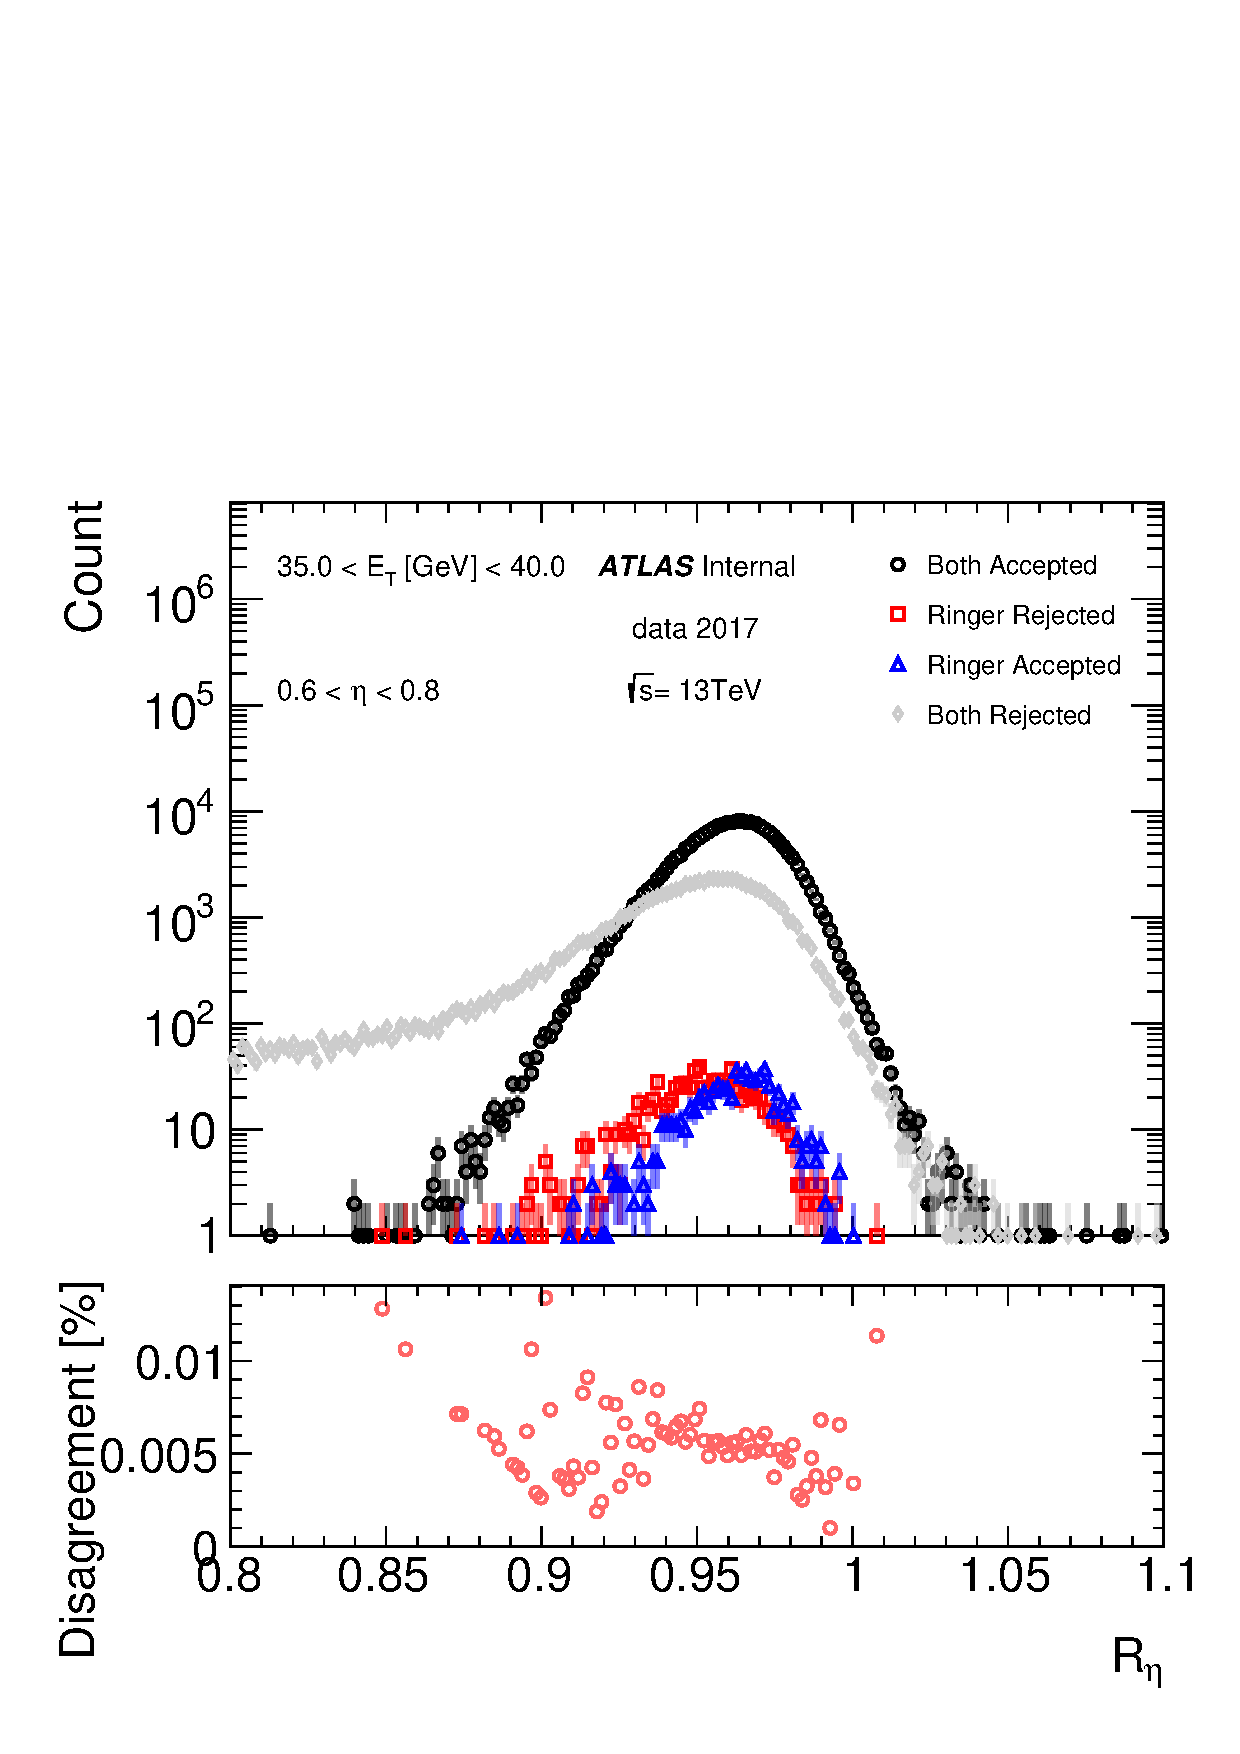
\includegraphics[width=\textwidth]{sections/05_analysis/figures/quadrant_plots/reta.pdf}
\caption{}
\label{fig:quadrant_calo_variables_30GeV_eta}
\end{subfigure}
%\hfill
\begin{subfigure}[c]{.49\textwidth}
\centering
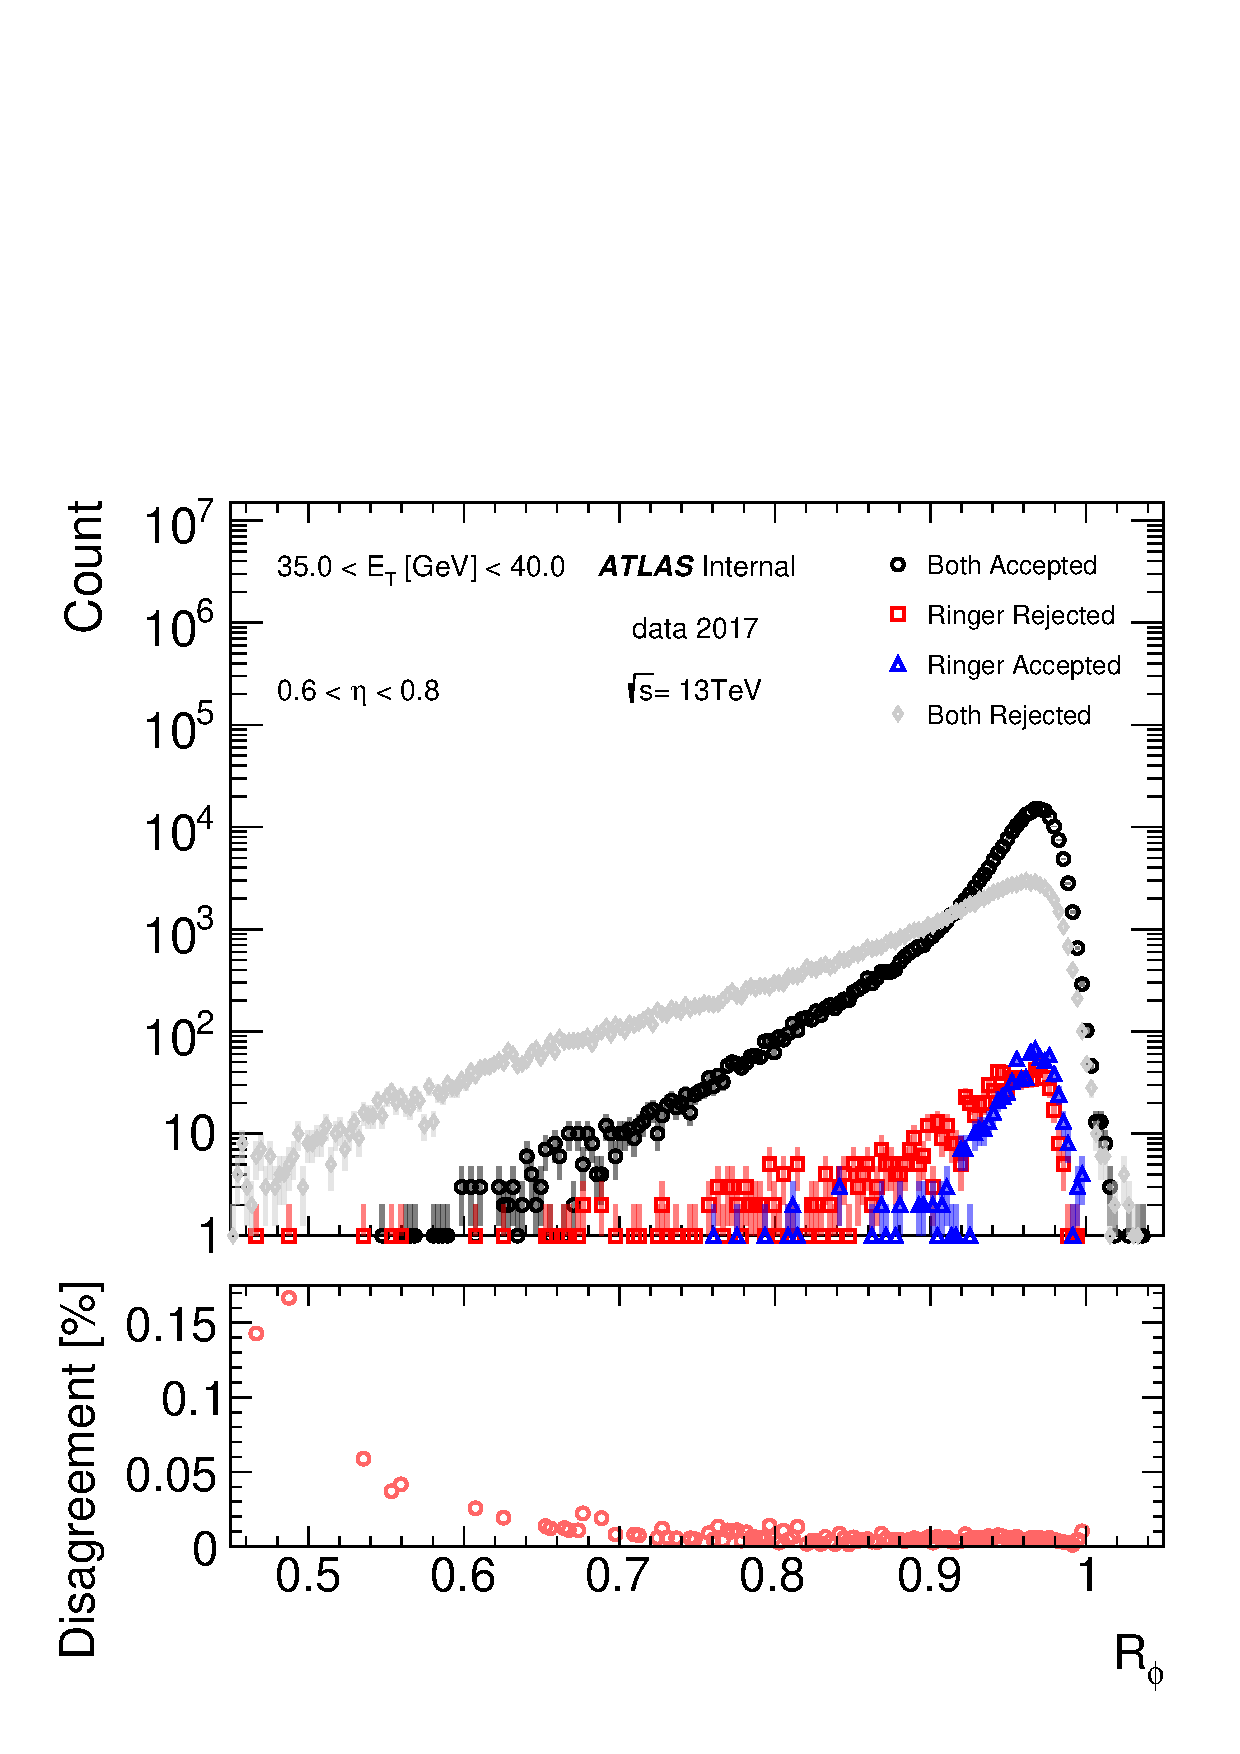
\includegraphics[width=\textwidth]{sections/05_analysis/figures/quadrant_plots/rphi.pdf}
\caption{}
\end{subfigure} 
%\end{figure}
%\begin{figure}[p]\ContinuedFloat
\begin{subfigure}[c]{.49\textwidth}
\centering
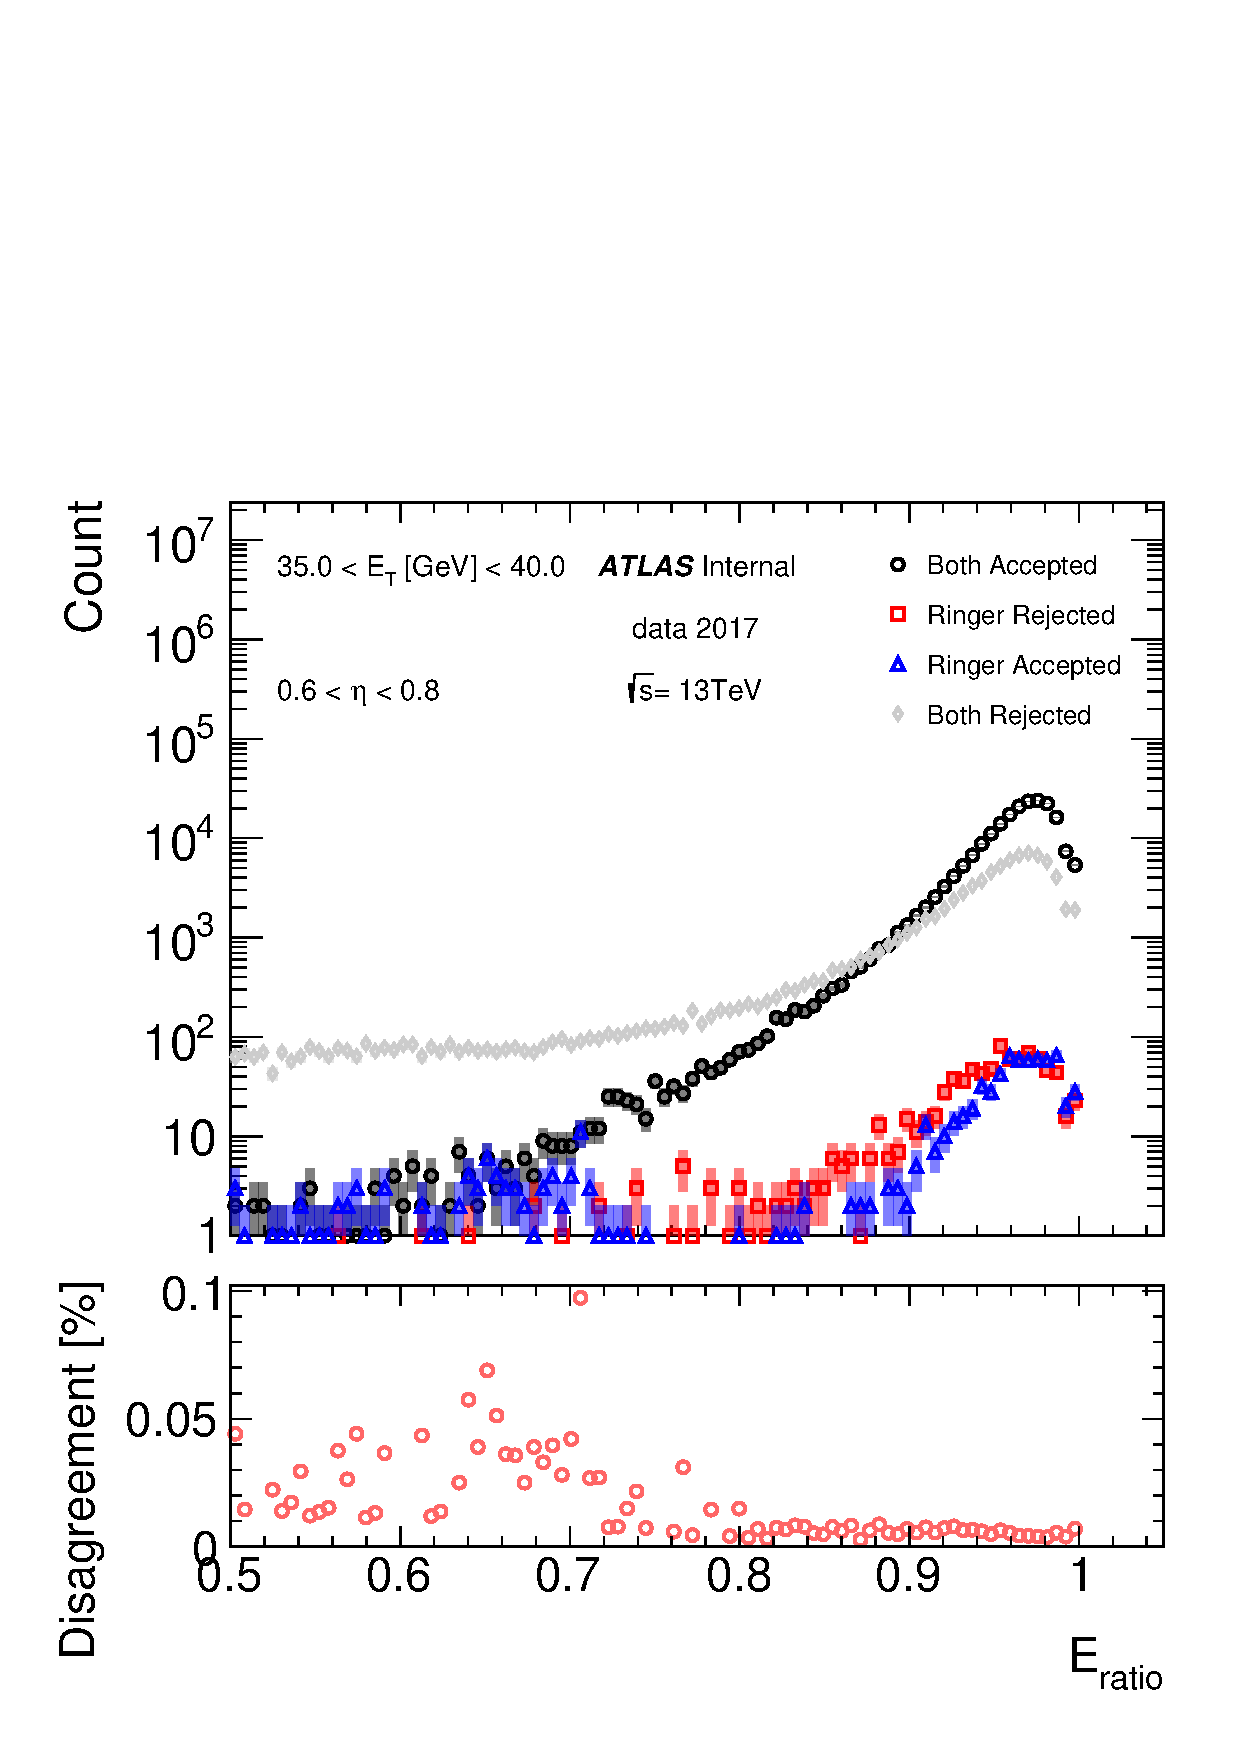
\includegraphics[width=\textwidth]{sections/05_analysis/figures/quadrant_plots/eratio.pdf}
\caption{}
\end{subfigure}
\hfill
\begin{subfigure}[c]{.49\textwidth}
\centering
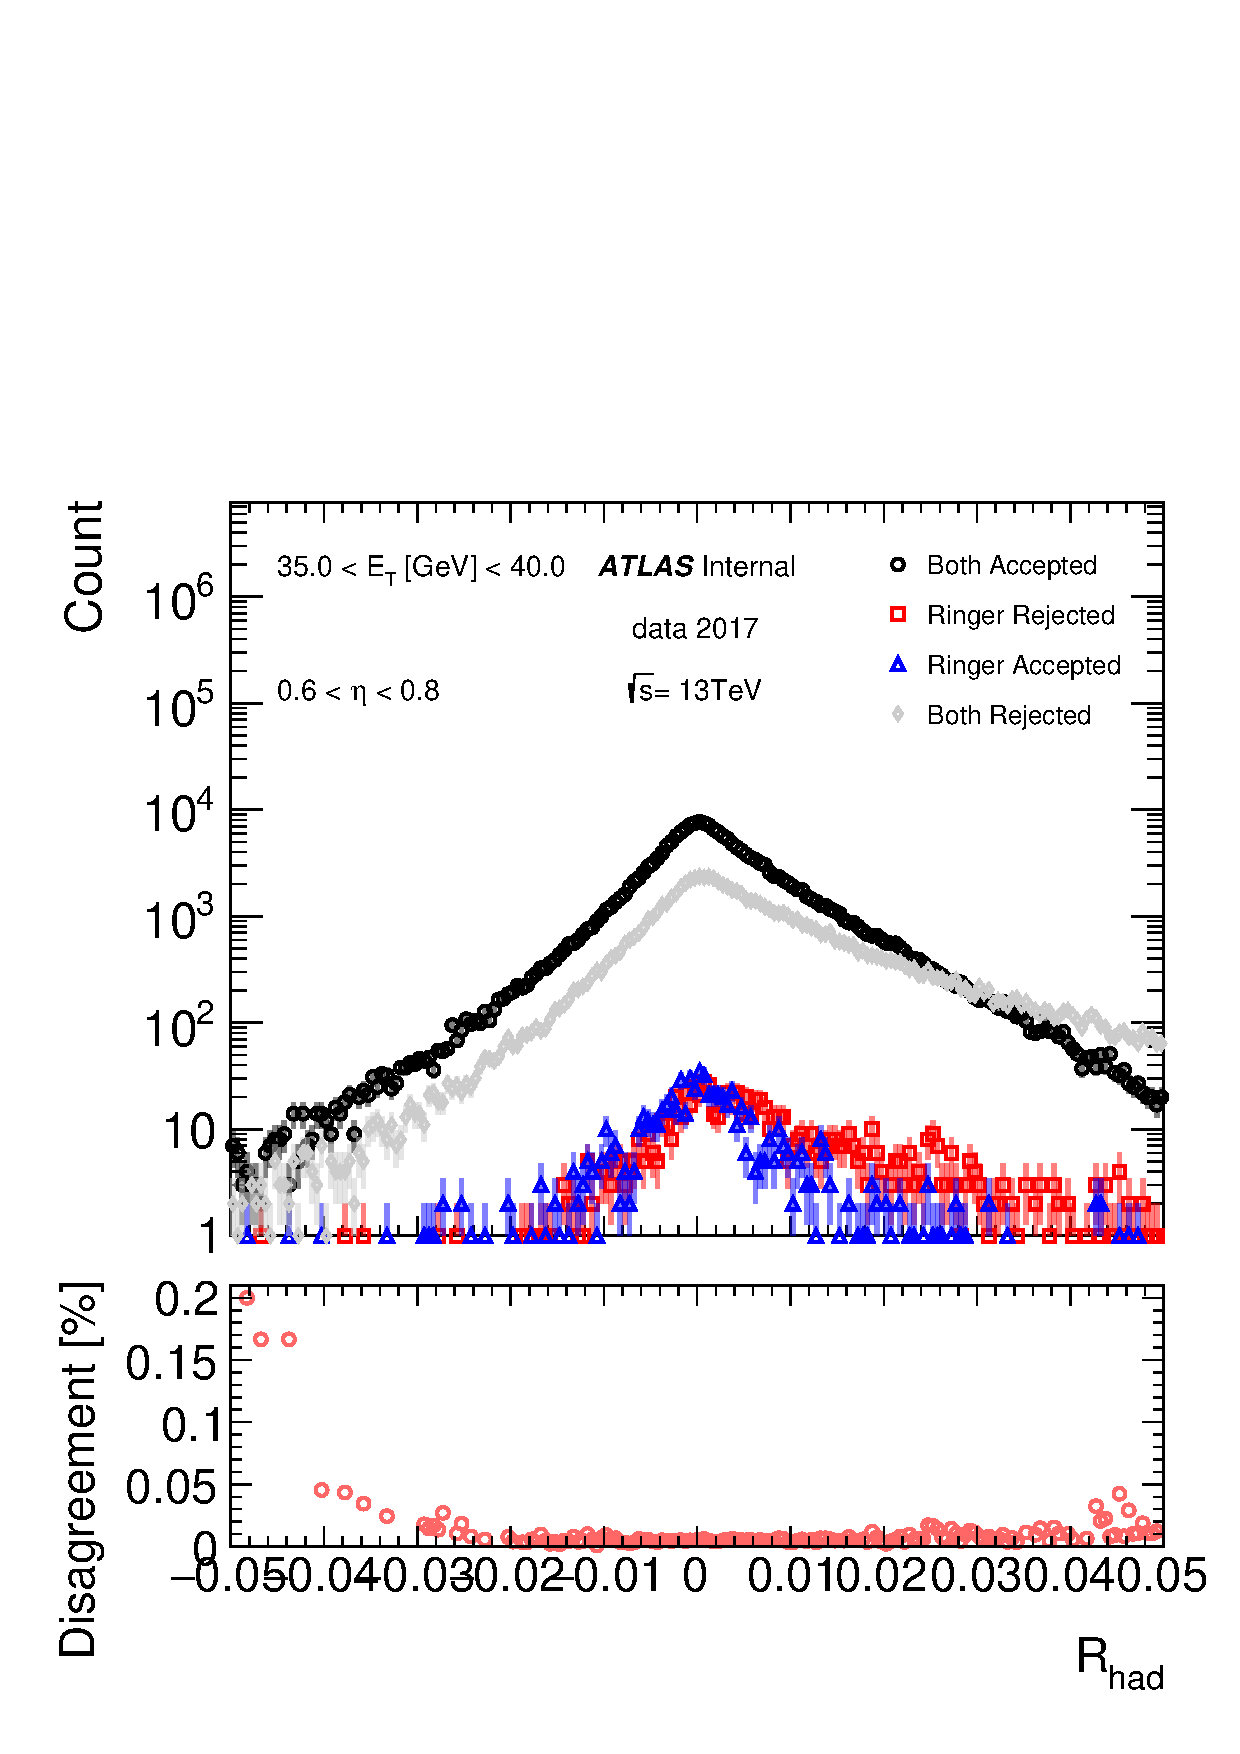
\includegraphics[width=\textwidth]{sections/05_analysis/figures/quadrant_plots/rhad.pdf}
\caption{}
\end{subfigure} \\


\caption{\label{fig:quadrant_calo_variables_30GeV}
	Quadrant analysis plots for the main offline-reconstructed
	calorimetry variables employed in the
	likelihood and for the $0.6<\abseta{}<0.8$ and
	$30<\et{}~[\text{GeV}]<35$ slices. 
	The top pad in each figure shows the raw number of observations for the four mutually exclusive cases: both with and without \rnn{}
	triggered (black); triggered only with \rnn{} (blue); triggered only without \rnn{} (red); neither one triggered (gray). The bottom pad contains disagreement as defined in the Equation \eqref{eq:disagreement}.
}
%Quadrant analysis plots for the offline-reconstructed
%calorimetry variables employed in the
%likelihood and \wstot{} for the $0.6<\abseta{}<0.8$ and
%$30<\et{}~[\text{GeV}]<40$ slices.}%
\end{figure}

Although similar behavior is shown for the other 
regions, the differences vary in strength in each \abseta{} region. As expected, 
the trigger does not show a dependence on ID variables, as shown in Figure~\ref{fig:quadrant_track_variables_30GeV} for $35<\et{}~[\text{GeV}]<40$, since the only distinction between them is the electron identification model operating in the \fastcalo{}.


\begin{figure}[h!tb]
%\centering
%\begin{subfigure}[c]{.49\textwidth}
\centering
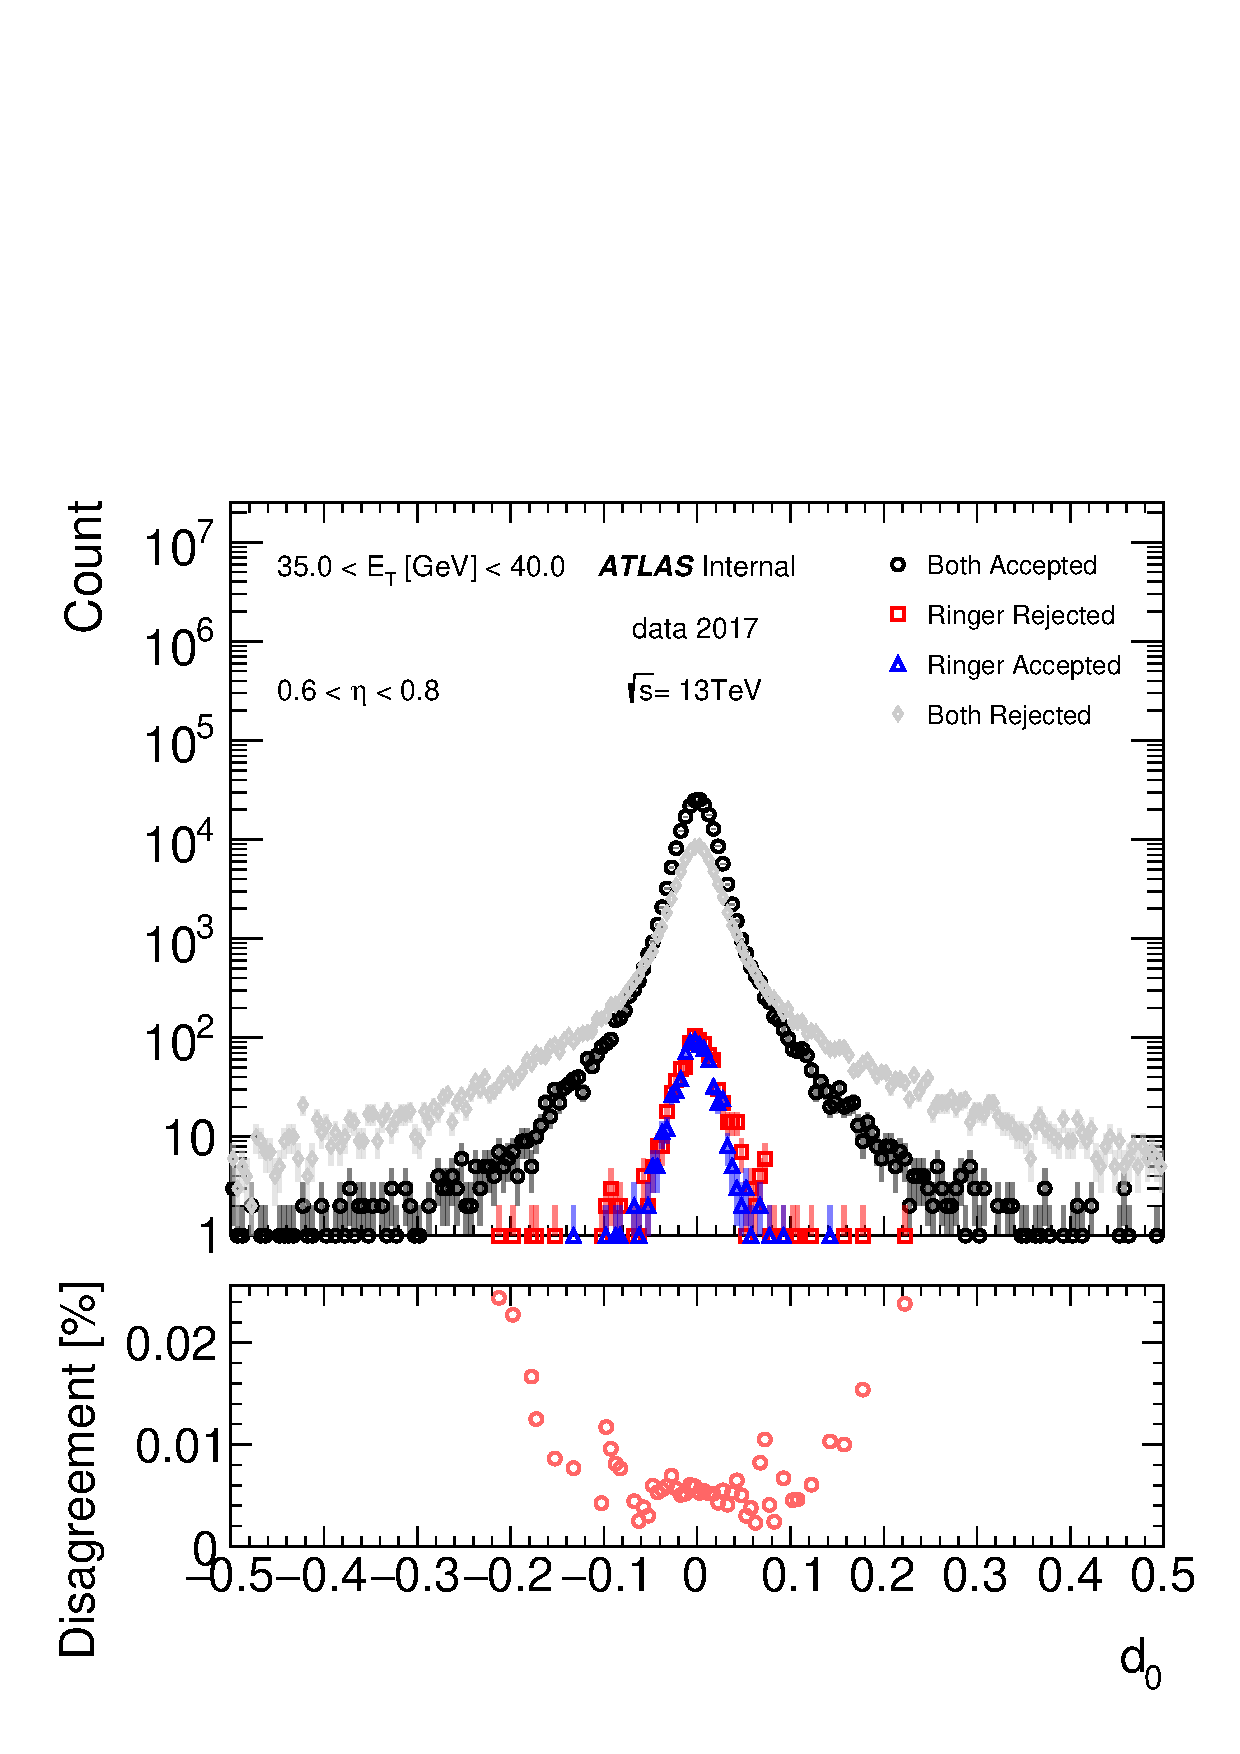
\includegraphics[width=.5\textwidth]{sections/05_analysis/figures/quadrant_plots/d0.pdf}

\caption{\label{fig:quadrant_track_variables_30GeV}
Quadrant analyses plots for the offline-reconstructed ID variable $d_0$ employed in the
likelihood for the $0.6<\abseta{}<0.8$ and $35<\et{}~[\text{GeV}]<40$ slice. The variable $d_0$ is defined as the transverse parameter of the impact point with respect to the collision beam.
}
\end{figure}






\FloatBarrier
\section[Homogeneity Tests]{Homogeneity Tests}\label{ssec:agreement}

In this 
analysis, the impact of using different triggers, \rnn{} and cut-based, on the likelihood algorithm is evaluated. This study requires a pair of duplicated triggers, composed by an $E_T > 28$ GeV isolated and Tight selection with and without the \rnn{}, operating online together. 
This analysis is performed using \Zee{} \tnp{} data, which were selected with the trigger requirement set to either one of the duplicated triggers for the tag, whereas the probe selection is invariably set to the offline \vloose{} criterion. This is the exact setup employed by ATLAS to derive the offline likelihood for electrons above \SI{15}{\GeV}~\cite{aaboud2019electron}. To benefit from the full 2017 statistics, data collected previous to the TS1 were also employed. In case the profiles are statistically identical, then it is expected that the \rnn{} trigger does not cause any relevant alteration in the derivation of the offline likelihood pdfs.  The statistical method for profile evaluation is described in Section~\ref{top:homogeneity_method} and the results are available in Section~\ref{top:agreement_homogeneity_results}.




\subsection{Method}\label{top:homogeneity_method}



The problem is approached based on homogeneity tests on histograms~\cite{homogeneity_test}, in order to check for (systematic) effects of the trigger configuration. It is based on a test originally developed by Pearson~\cite{pearson1911probability} and popularly employed in many fields beyond High Energy Physics (HEP), e.g. social sciences~\cite{wickens2014multiway} and health~\cite{ma2015homogeneity}, usually labelled as contingency or consistency tests.

In order to benefit from the test without having to customize it to the ATLAS particular analysis setup, the following method was followed. First, the data was spitted into two
statistically independent groups attempting to keep data taking conditions as
similar as possible by successively taking data to each group from small
consecutive periods.

Ideally, it would be desired to split data using luminosity
blocks for achieving nearly the same conditions. However, technical limitations
constrained the period to larger time scales, hence allowing the test to
indicate that the two groups are originating from different populations due to
confounding variables. Either way, it does not affect the goal of this assessment. 
By comparing the p-values of the two groups, it is possible to evaluate how the different configuration affects the likelihood of the profiles to be drawn from the same distribution. 


If the p-values\footnote{The p-value here is defined by: $P-value \approx f(x, k) = \frac{1}{2^{k/2}\Gamma(k/2)}x^{k/2 -1}e^{-x/2}$} have negligible fluctuations with respect to the values obtained by the tests comparing the same triggers, then the systematic effect in the profiles is negligible with respect to half\footnote{Once each group is using nearly half of the integrated luminosity.} of the statistics available.



To provide a better insight on possible distortions, the corresponding $\chi$
individual contributions of each group are computed allowing them to freely
oscillate through the positive and negative axis with

\begin{equation}
  \chi_{i,j}^{s} = \frac{(r_{i,j} - b_{i,j})}{\sqrt{b_{i,j}}},
  \label{eq:signed_chi}
\end{equation}

\noindent where $r_{i,j}$ ($b_{i,j}$) is the number of observations collected by
the trigger with (without) \rnn{} in $j$th histogram bin and in the $i$th
$\et{}\times\abseta{}$ region.


\subsection{Results}\label{top:agreement_homogeneity_results}




Regardless of the trigger configuration, the p-values of the homogeneity tests between the two groups result in similar values. In other words, the fluctuations in the profiles are mainly dominated by statistical fluctuations, with no sign of systematic effects due to the trigger configuration. 

Similar behavior is observed for the ID and calo-ID variables. The Figure~\ref{fig:groups_homogeneity_calo} shows the residuals when considering the histogram obtained with data collected by the trigger without \rnn{} for the first arbitrary group as a reference. The residuals are dominated by statistical fluctuations, which are within the expectations from homogeneity hypothesis for most variables and regions.


\begin{figure}[b]
\begin{center}
\begin{subfigure}[c]{.48\textwidth}
\centering
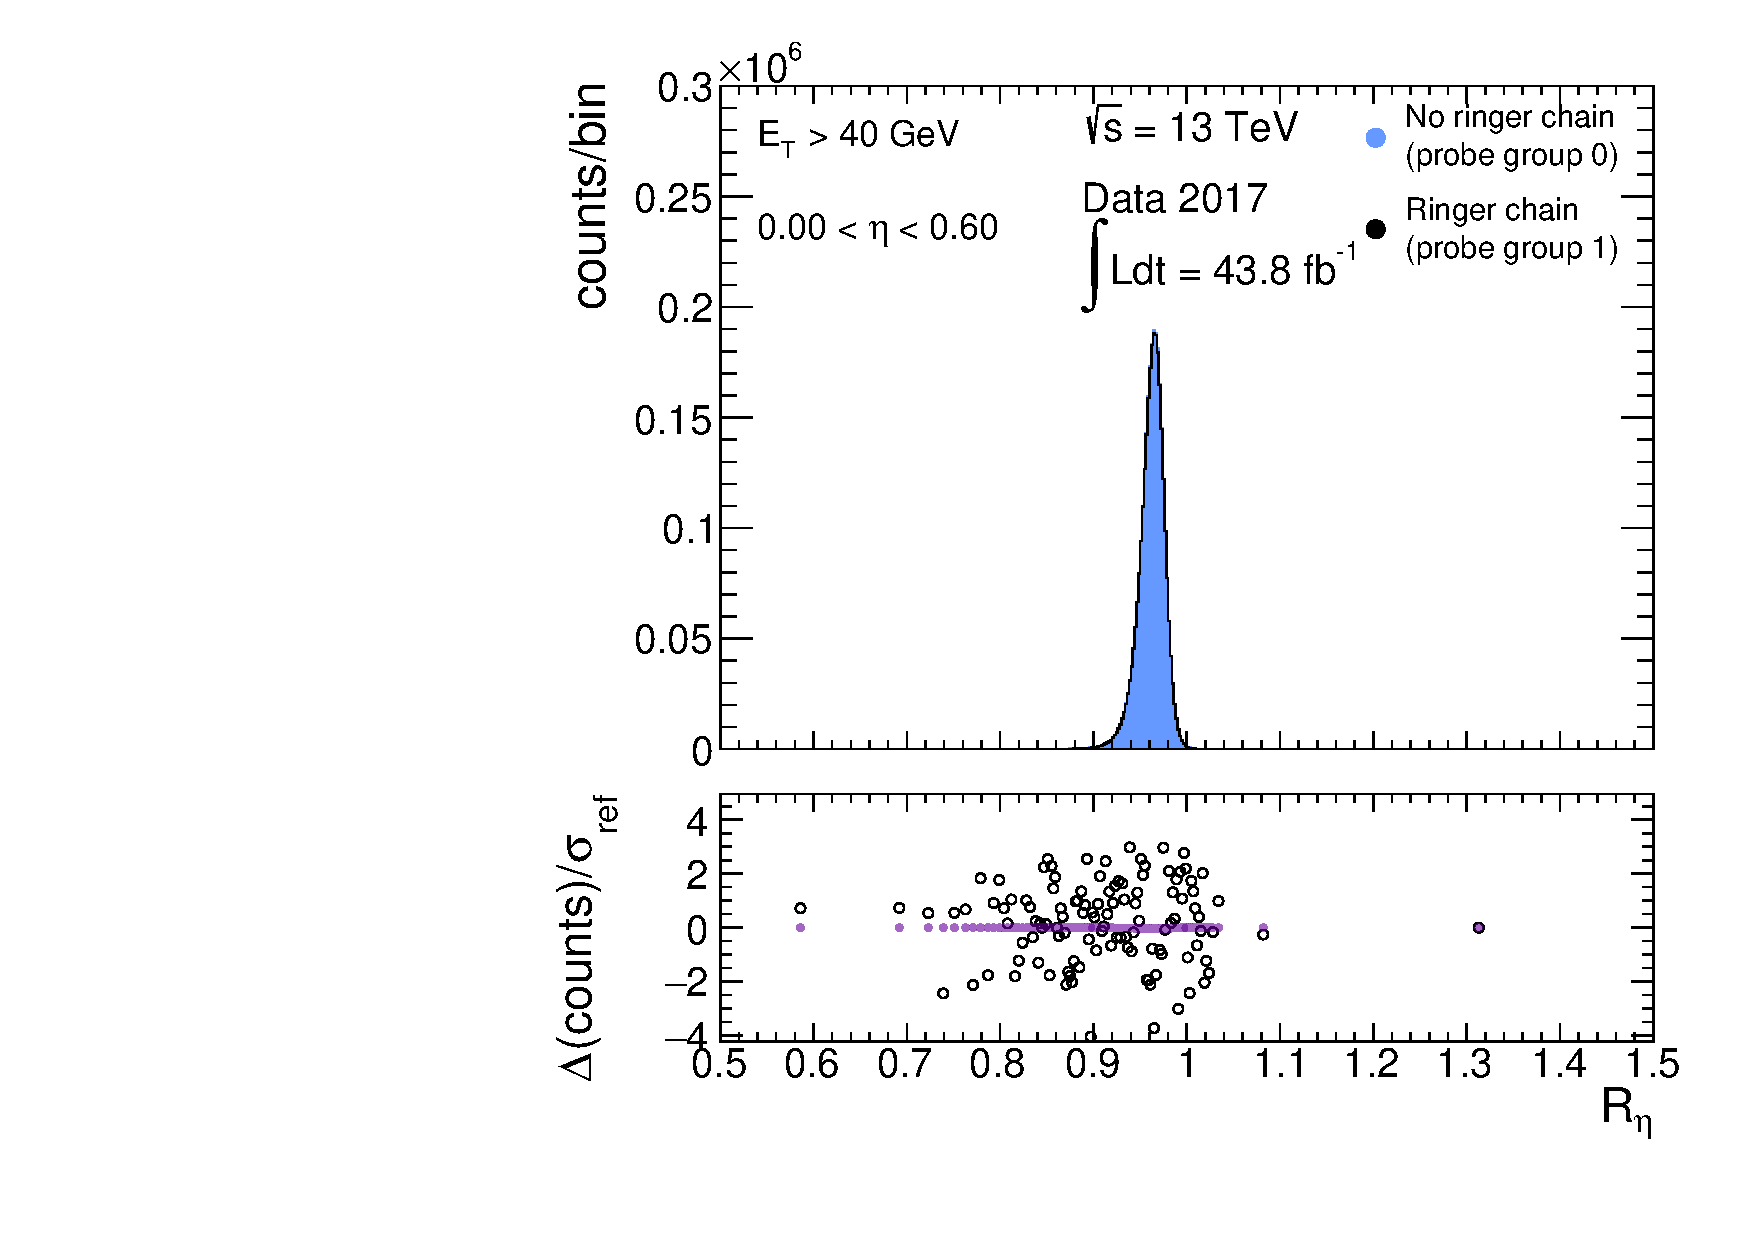
\includegraphics[width=\textwidth]{sections/05_analysis/figures/noAdjustment/el_reta_et40eta0_00_sigma_base_new.pdf}
\caption{}%

\end{subfigure}
\hfill
\begin{subfigure}[c]{.48\textwidth}
\centering
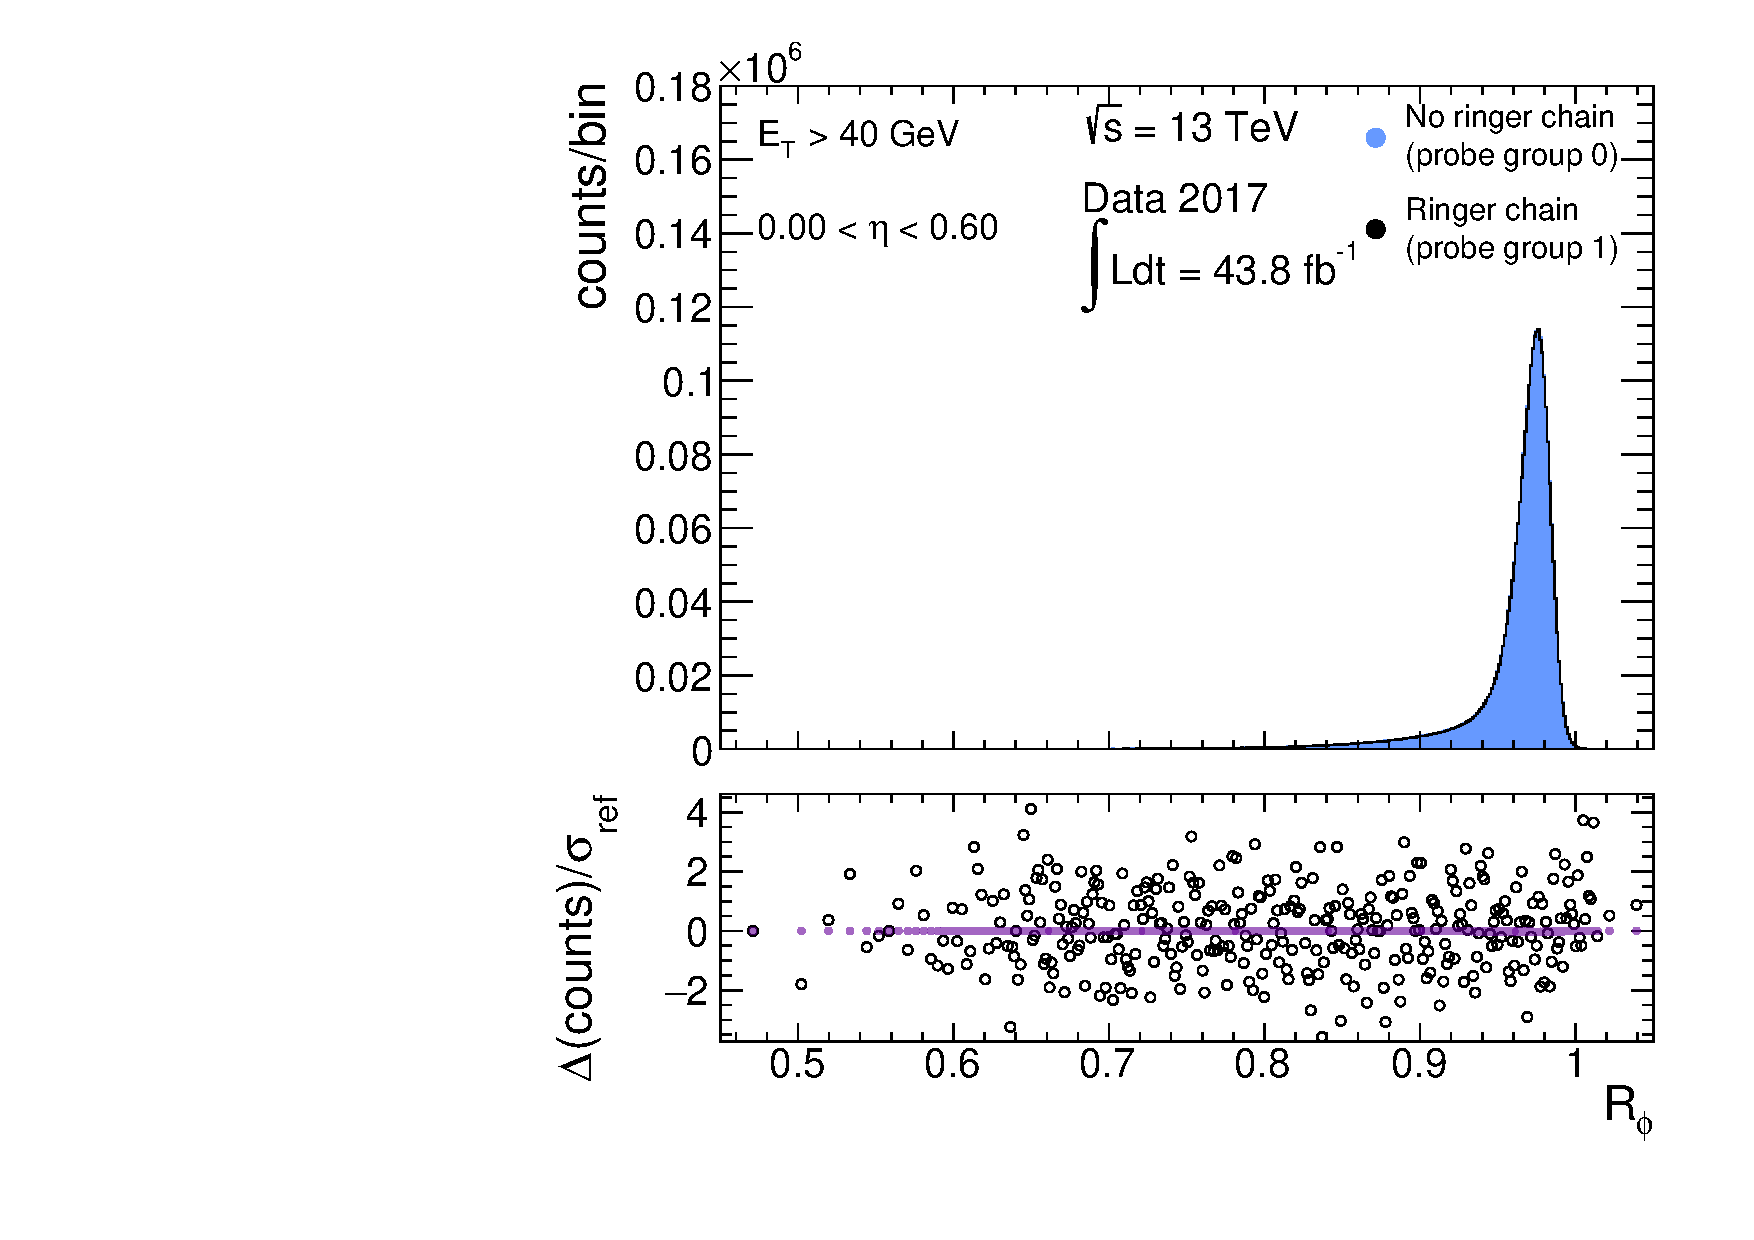
\includegraphics[width=\textwidth]{sections/05_analysis/figures/noAdjustment/el_rphi_et40eta0_00_sigma_base_new.pdf}
\caption{}%

\end{subfigure} \\
\begin{subfigure}[c]{.48\textwidth}
\centering
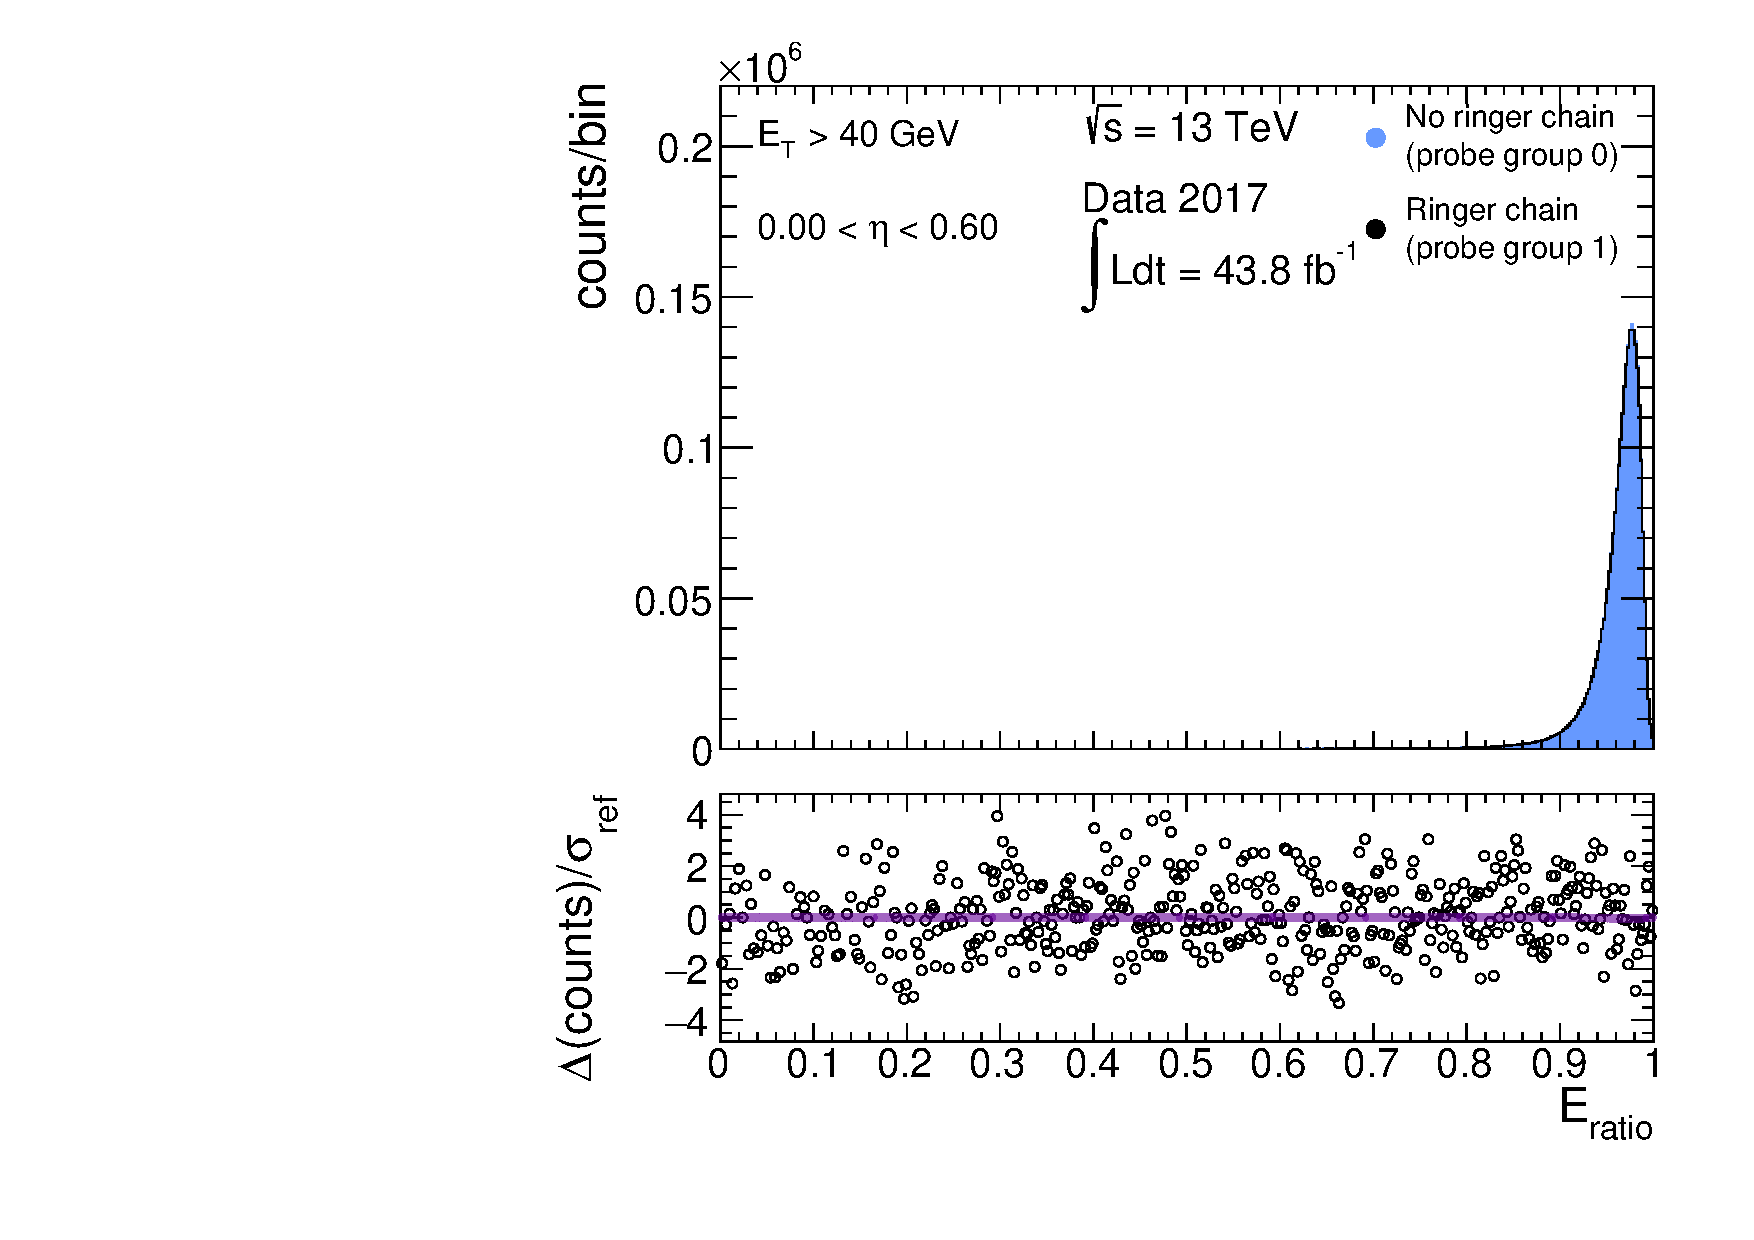
\includegraphics[width=\textwidth]{sections/05_analysis/figures/noAdjustment/el_eratio_et40eta0_00_sigma_base_new.pdf}
\caption{}%

\end{subfigure}
\hfill
\begin{subfigure}[c]{.48\textwidth}
\centering
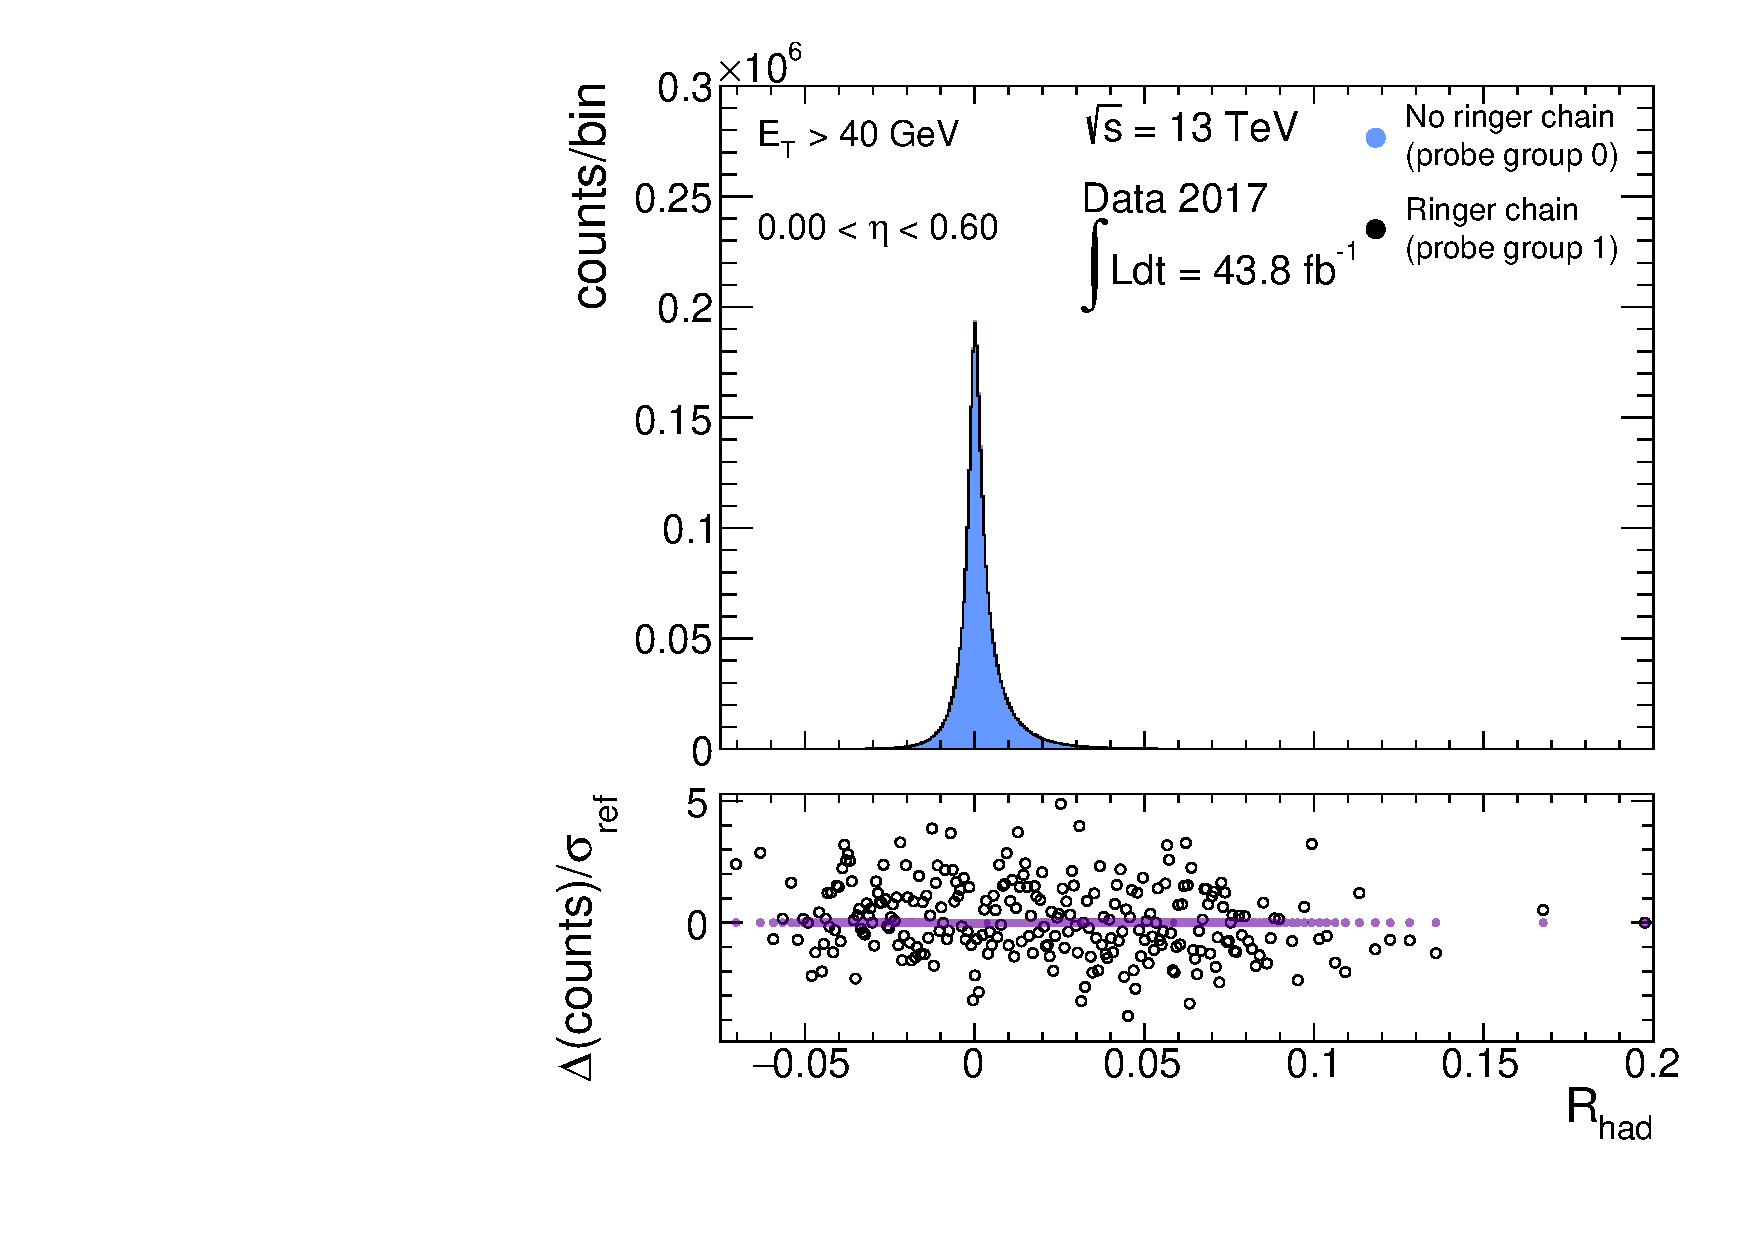
\includegraphics[width=\textwidth]{sections/05_analysis/figures/noAdjustment/el_rhad_et40eta0_00_sigma_base_new.pdf}
\caption{}%

\end{subfigure} \\
\caption{%
	Top: \reta, \eratio, \rphi, \rhad histogram profiles for the calorimetry variables employed in the offline likelihood in the $\et>\SI{40}{\GeV}$ and $0.00<\abseta{}<0.80$ regions using data collected by
	triggering without \rnn{} in the first arbitrary data group
	(blue area) and data collected by triggering with \rnn{} in the second
	arbitrary data group (black line).  Bottom: residual contributions using as
	statistics $\chi^s$ (equation~\ref{eq:signed_chi}, in black) and the expected
	model for no distortion given by the $\chi^s$ residuals w.r.t.\@ the
	reference.
}%
\label{fig:groups_homogeneity_calo}
\end{center}
\end{figure}%


\FloatBarrier
